\section{Methods}
This section provides a detailed description of the advanced statistical methods used in the analysis, including their mathematical definitions and references to relevant literature. Basic concepts are assumed to be known and are not covered here.

\subsection{Missing Value Imputation}

The dataset contains 1,797 Netflix movies and 197 Disney+ movies with missing \texttt{Age} values, totaling approximately 2,000 records. Dropping these entries would result in a significant loss of valuable data, making this approach unsuitable. Therefore, imputing the missing values is necessary.
We applied both \textit{mode imputation} and \textit{KNN imputation} methods, and the analysis will demonstrate why KNN imputation proves to be the more effective approach.

\subsubsection{Ordinal Encoding of Age Variable}

We applied \textit{ordinal encoding} to the \texttt{Age} variable to convert its categorical values (e.g., \texttt{7+}, \texttt{13+}, \texttt{18+}, \texttt{All}) into corresponding numeric values (e.g., \texttt{7}, \texttt{13}, \texttt{18}, \texttt{0}). This transformation was necessary to enable statistical analysis and visualization, as numerical data is required for most quantitative methods.

\textit{Ordinal encoding} is a technique used to convert categorical data with an inherent order into numerical form. In this case, higher values represent age suitability for older audiences, maintaining the natural hierarchy of the categories. \cite{von_eye1996categorical} This ensures that the encoded data reflects the meaningful relationships between age groups. \textbf{Figure~\ref{fig:age_encoding}} depicts the effect of this encoding.

\begin{figure}[H]
    \centering
    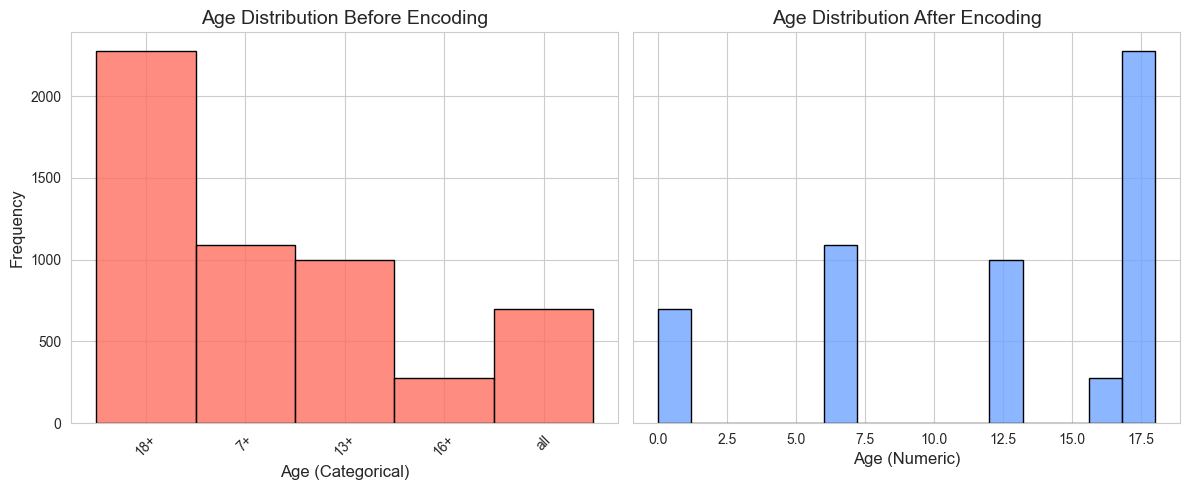
\includegraphics[width=\textwidth]{encode_age.png}
    \caption{Age Distribution Before and After Encoding}
    \label{fig:age_encoding}
\end{figure}

\subsubsection{Mode Imputation}

\textbf{Mode imputation} fails to handle the \texttt{Age} variable effectively, as seen in \textbf{Figure ~\ref{fig:mode_imputation}}. By replacing all missing values with the most frequent age (the mode), it creates an \textbf{artificial spike} in the distribution, leading to an unnatural concentration around a single age group. This oversimplifies the data and skews the original variability, as illustrated in the sharp peak in the \textit{After Mode Imputation} plot.

In contrast, the \textit{Before Mode Imputation} plot shows a natural spread across multiple age groups, reflecting a \textbf{multimodal distribution}. Mode imputation does not respect this diversity, making it unsuitable for data with multiple natural peaks. A more appropriate method, such as \textbf{KNN imputation} (refer to \autoref{appendix:knn}), maintains the original distribution by using similar records to estimate missing values.

\begin{figure}[H]
    \centering
    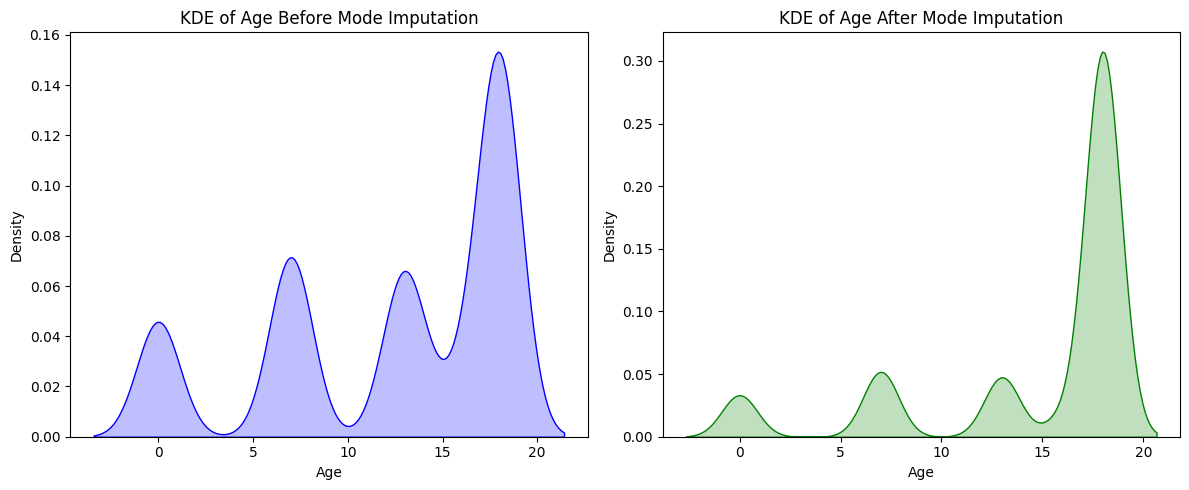
\includegraphics[width=\textwidth]{mode.png}
    \caption{Impact of Mode Imputation on Age Distribution: KDE Plot (refer to \autoref{appendix:kde})}
    \label{fig:mode_imputation}
\end{figure}

\subsubsection{KNN Imputation}

\textbf{Figure~\ref{fig:knn_imputation}} shows that KNN preserves the natural spread and multimodal peaks of the \texttt{Age} distribution. Unlike mode imputation, which created an artificial spike by concentrating missing values around a single age group, KNN imputation fills missing values based on similarity with neighboring records. This approach respects the original variability and maintains a more realistic distribution, as seen in the smooth, continuous curve of the \textit{After KNN Imputation} plot. This makes KNN a better choice for datasets with diverse categories, like age ratings.

\begin{figure}[H]
    \centering
    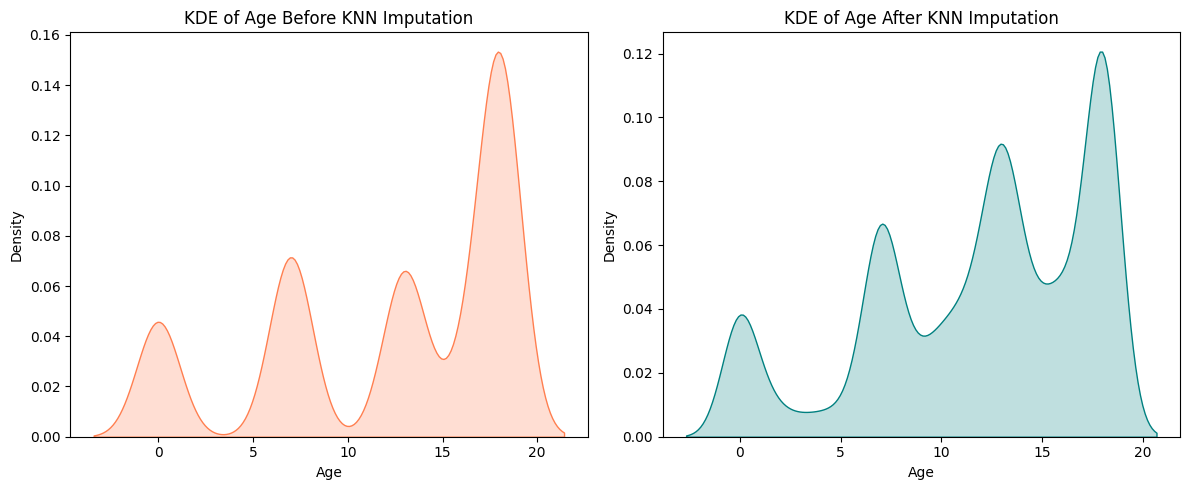
\includegraphics[width=\textwidth]{knn.png}
    \caption{KDE Plot of Age Distribution Before and After KNN Imputation}
    \label{fig:knn_imputation}
\end{figure}

\subsection{Visualization}

After handling the missing values, we calculated the \textbf{mean} and created \textbf{box plots} (refer to \autoref{appendix:box_plot}) for the \texttt{Age} and \texttt{Rotten Tomatoes} variables to visualize their distributions. These measures provide a summary of central tendency and variability.

\begin{figure}[H]
    \centering
    \begin{subfigure}[t]{0.48\textwidth}
        \centering
        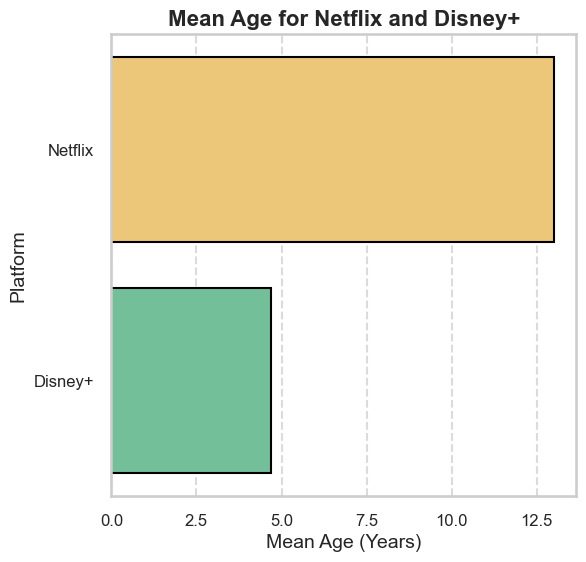
\includegraphics[width=\textwidth]{mean_age.png}
        \caption{Mean Age Ratings for Netflix and Disney+}
        \label{fig:mean_age}
    \end{subfigure}
    \hfill
    \begin{subfigure}[t]{0.48\textwidth}
        \centering
        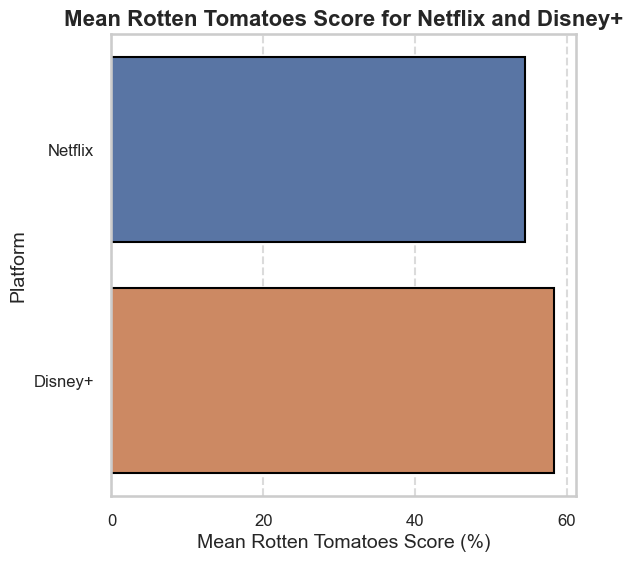
\includegraphics[width=\textwidth]{mean_tomato.png}
        \caption{Mean Rotten Tomatoes Scores for Netflix and Disney+}
        \label{fig:mean_tomato}
    \end{subfigure}

    \vspace{0.5cm}

    \begin{subfigure}[t]{0.48\textwidth}
        \centering
        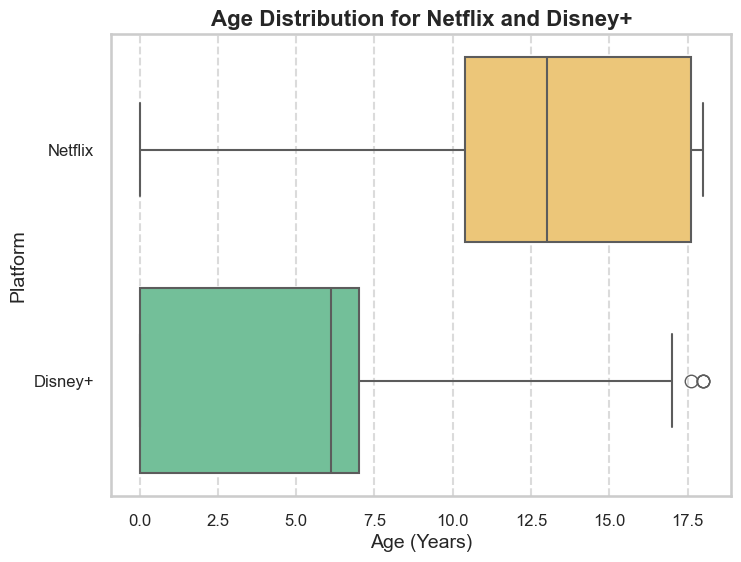
\includegraphics[width=\textwidth]{box_age.png}
        \caption{Age Distribution for Netflix and Disney+ (Box Plot)}
        \label{fig:box_age}
    \end{subfigure}
    \hfill
    \begin{subfigure}[t]{0.48\textwidth}
        \centering
        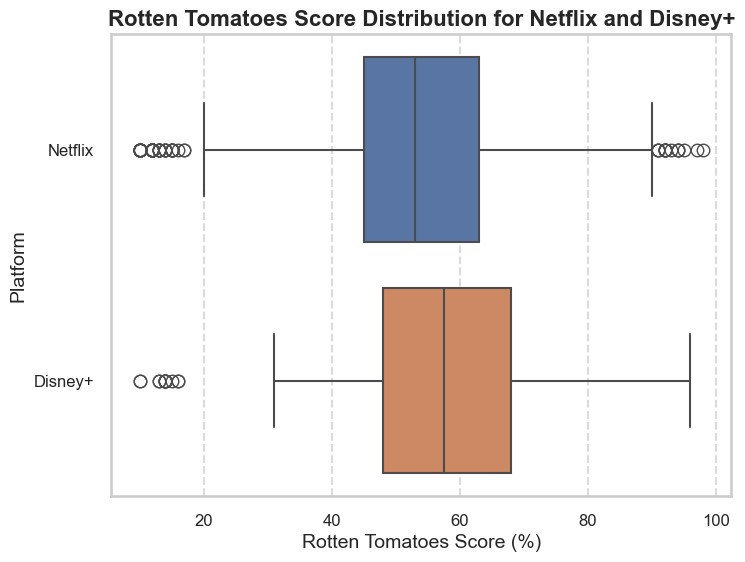
\includegraphics[width=\textwidth]{box_tomate.png}
        \caption{Rotten Tomatoes Score Distribution for Netflix and Disney+ (Box Plot)}
        \label{fig:box_tomato}
    \end{subfigure}

    \caption{Visualizations of Age Ratings and Rotten Tomatoes Scores for Netflix and Disney+}
    \label{fig:age_tomato_plots}
\end{figure}

\vspace{0.5cm}

\textbf{Figure~\ref{fig:mosaic_age}} features a mosaic plot regarding age categories. A \textbf{Mosaic Plot} is a visual tool used to analyze the relationships between categorical variables by representing them as proportional rectangles. Each rectangle's area corresponds to the frequency or relative frequency of a particular category combination, making it easy to compare distributions across groups. This plot is particularly useful for identifying patterns, dependencies, and disparities in data. In the given plot, it compares age ratings (0-7, 7+) across Disney+ and Netflix, highlighting which platform dominates specific age categories.

\begin{figure}[H]
    \centering
    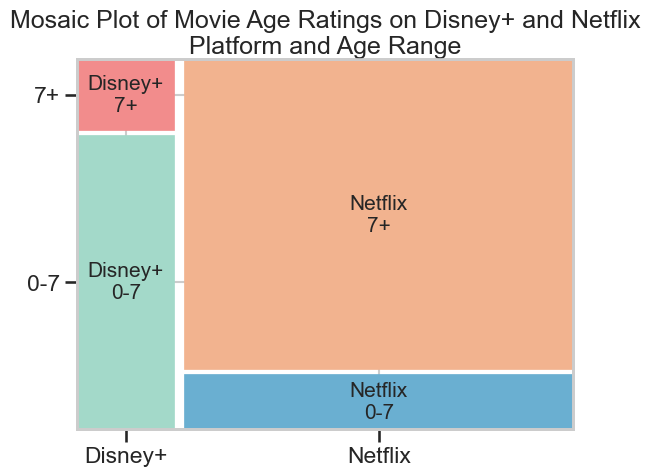
\includegraphics[width=0.5\textwidth]{mosaic.png}
    \caption{Mosaic Plot of Age Ratings Distribution Across Disney+ and Netflix}
    \label{fig:mosaic_age}
\end{figure}

\textbf{Figures~\ref{fig:rig_scatter_plots}} analyze Rotten Tomatoes scores for Netflix and Disney+. The Ridgeline Plot provides an overview of score distributions, highlighting density, central tendency, and variability, enabling clear platform comparisons by stacking multiple density plots. The Scatter Plot with Jitter complements this by displaying individual scores, reducing overlap with jitter to reveal clustering and outliers. Together, these visualizations offer both aggregated insights and granular details, providing a comprehensive understanding of the data. \cite{Waskom2021}

\begin{figure}[H]
    \centering
    \begin{subfigure}[t]{0.48\textwidth}
        \centering
        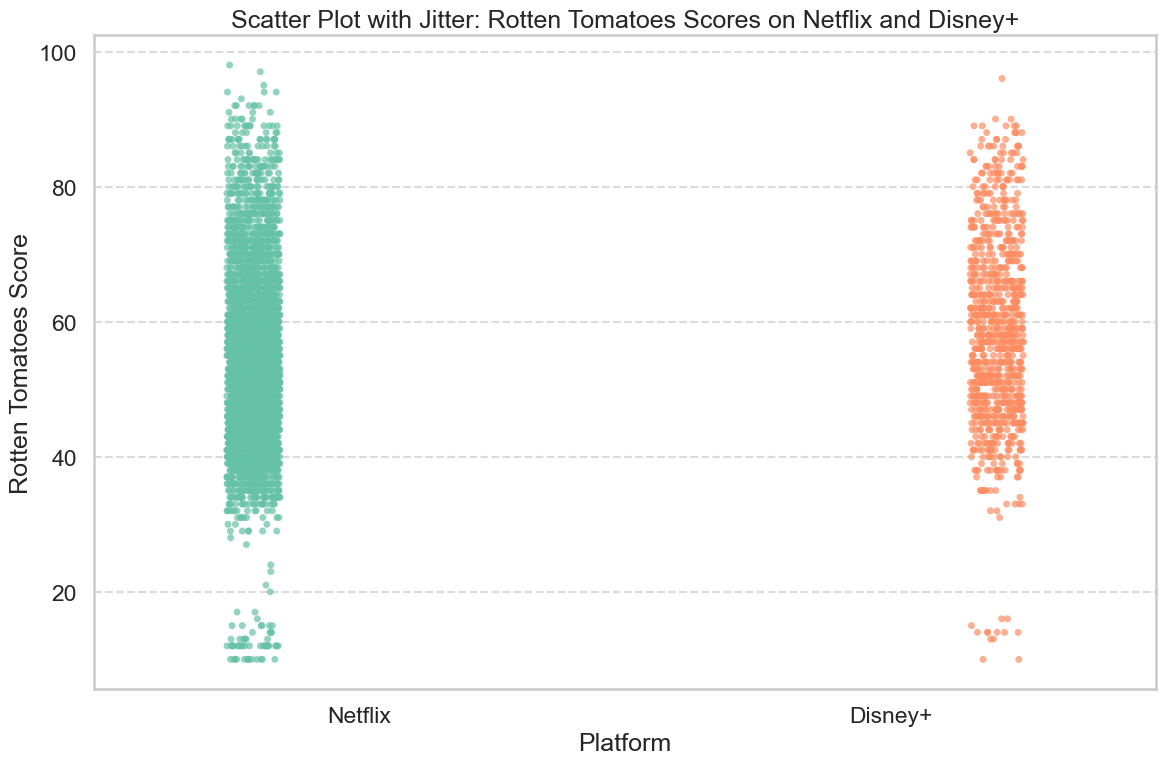
\includegraphics[width=\textwidth]{scatter.png}
        \caption{Scatter plot}
        \label{fig:scatter}
    \end{subfigure}
    \begin{subfigure}[t]{0.48\textwidth}
        \centering
        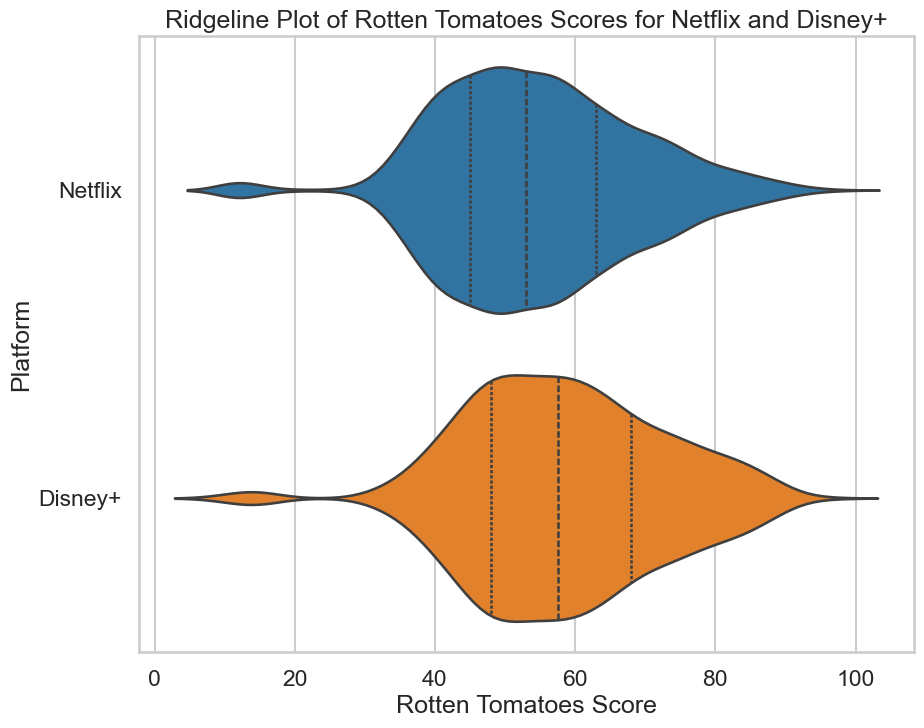
\includegraphics[width=\textwidth]{ridgeline.png}
        \caption{Ridgeline Plot}
        \label{fig:ridgeline}
    \end{subfigure}
        \caption{Rotten Tomatoes Scores distribution visualized}
    \label{fig:rig_scatter_plots}
\end{figure}
